\section{Introduction}\label{sec:intro}
The success of deep neural networks (DNN) have been proven in many applications, such as object detection~\citep{liu2016ssd,ren2015faster,girshick2015fast}, image classification~\citep{he2016deep,szegedy2015going,simonyan2014vgg,krizhevsky2012imagenet}, semantic segmentation~\citep{noh2015learning,pohlen2017full,girshick2014rich,long2015fcn}, visual question answering~\cite{noh2016image,malinowski2015ask} and natural language processing~\citep{graves2013speech}.
Recently, deep neural models have become deeper and deeper to provide better accuracy~\cite{resnet,googlenet,mobilent}.
%for the large data set, such as the famous ImageNet\citep{deng2009imagenet}, to achieve a higher accuracy. For example, the number of parameters of VGG-16 \citep{simonyan2014vgg} is as high as $138\times10^6$, and the storage capacity of this model reaches 528MB. 
Large DNN models bring in many challenges for real life applications, especially difficulties for the deployment on resource-limited platforms, such as mobile and Internet-of-Thing (IoT) devices. There are three critical challenges for deploying DNNs to resource-limited platforms: 1) computing capability; 2) energy consumption; 3) storage capacity.
Network compression refers to a series of processes to compress a large model into a smaller one, which can solve the challenges of deploying large network models to resource-limited devices.
It is to reduce the redundancy of the model, for example redundant weights and features, and remain its performance in terms of execution efficiency and accuracy. 

\begin{figure}[!]
    \centering
    \subfloat[Cifarnet conv1]{
        \label{Cifarnet-conv1}
        \begin{minipage}[t]{0.24\textwidth}
        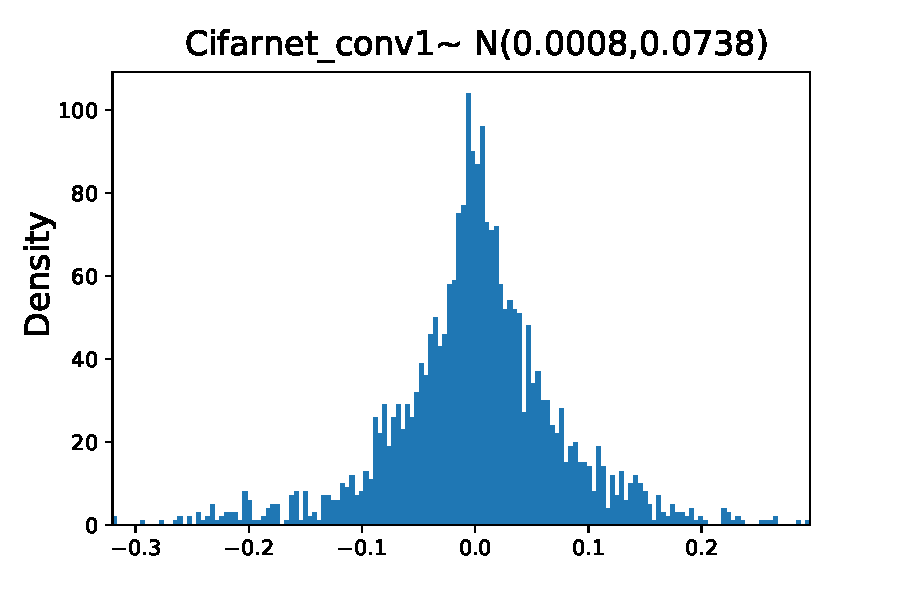
\includegraphics[width=1\textwidth]{ActualWeights/Cifarnet/conv1/Distribution.pdf}
        \end{minipage}
    }
    \subfloat[Resnet-18 conv1]{
        \label{Resnet-18-conv1}
        \begin{minipage}[t]{0.24\textwidth}
        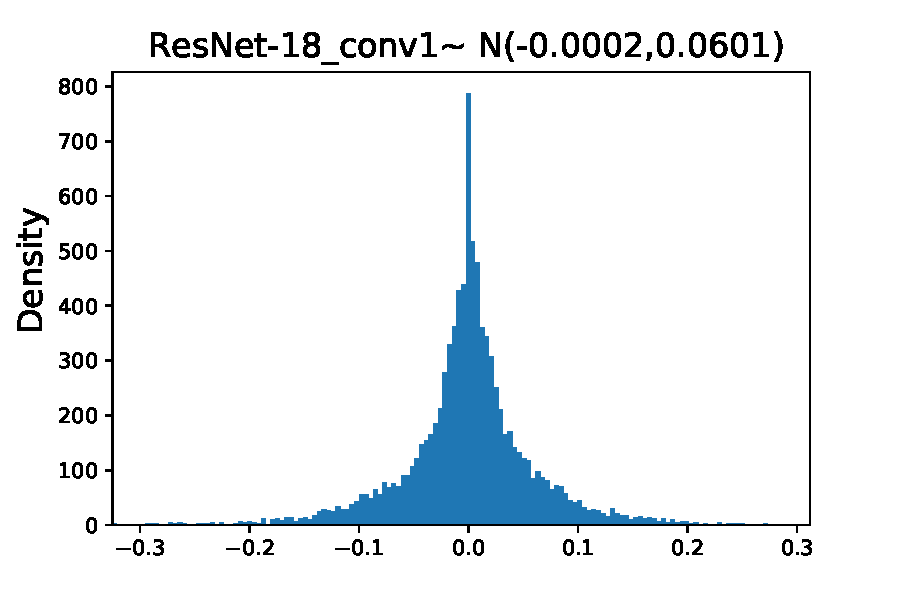
\includegraphics[width=1\textwidth]{ActualWeights/Resnet-18/conv1/Distribution.pdf}
        \end{minipage}
    }
    \caption{The weights of first convolutional layer of cifarnet \citep{krizhevsky2009learning} and Resnet-18 \citep{he2016deep}.}
    %approximately obeying the normal distribution.}
    \label{fig:nd}
    \vspace{-4mm}
\end{figure}

Data quantization is one of the most commonly used methods for network compression~\cite{han2015deep}. 
It aims to reduce the bitwidth of the co-efficient data with the tolerance of a certain loss of the precision for the original data~\citep{zhou2016dorefa,hubara2016binarized,han2015deep}.
% , and achieve a trade-off between the bit width and the data loss.
The low bit width of the representation of data directly reduces the memory footprint of the model, energy consumption and computing requirements~\cite{gysel2016hardware,rastegari2016xnor}.
Consequently, the quantized models can be deployed into resource-limited devices easily~\citep{zhou2016dorefa,ghasemzadeh2018rebnet}.

Current data quantization methods for DNN compression are mostly based on empirical guidance~\cite{} and experimental verification~\cite{}, lack of theoretical analysis and support.
Existing solutions encountered some difficulties: bad trade-off, depending on manual parameter settings and ignoring the distribution of the raw data.
\paragraph{Bad trade-off}: 
The current methods are hard to achieve the trade-off between bit width and data loss\footnote{Data loss refers to the loss of data before and after quantization}. Binary \citep{hubara2016binarized} or Ternary \citep{TWNs} have the fixed low bit width (1/2bit), but a large data loss. The fixed point quantization \citep{gysel2016hardware} can achieve a low data loss, but hard to achieve a low bit width.
\paragraph{Manually setting parameters}: 
Most existing data quantization methods squeeze the data to be quantized within a fixed number of bits by introducing a scaling factor to change the data range. The scaling factor is usually selected based on manual design, by data statistics and experimental verifications of the trained results. 
\paragraph{Ignoring data distribution}: 
Representative works such as Dorefanet \citep{zhou2016dorefa} and Hardware \citep{gysel2016hardware} have quantized the weights to different bit widths and given a well experimental results, but they did not explicitly state the conditions that the input data needs, and hard to guarantee the effectiveness for all situations. 

According to the derivation hypothesis \citep{nasrabadi2007pattern} of the L2 regular term, the weights of the layers in a DNN \textcolor{red}{approximately} follow normal distribution. 
As an instance, Figure~\ref{fig:nd} shows the distribution of the weights of the first layer from two classical models.
%However, existing quantization methods failed to consider this feature and lost the opportunity for analytical quantization during model training.
The ignorance of the distribution of the data in the theoretical analysis brings worse quantization performance.

In order to provide better trade-off between bit width and data loss and quantitatively analysis the loss of the data quantization, in this paper, we propose an ultra-low data loss quantization method called $\mu$L2Q. 

Our method considers the distribution of the data to be quantized, and guarantees 
that any data set that satisfy the distribution hypothesis can achieve the ultra-low data loss with our quantization.
% In addition, our method can achieve ultra-low data loss for any bitwidth quantization.
We summarize our contributions as the following:
%\textcolor{red}{(Cong: the contributions need further polishing; will come back later)}
\begin{itemize}
    \item We propose an effective ultra-low loss quantization  method  ($\mu$L2Q)  which  can  find  the  optimal discrete subspace from the contiguous space, minimizing the loss of data  mapping with our quantitative analysis.
    \item \textcolor{red}{Giving the optimal $\lambda$ set for different  bit  widths, ensuring that the optimal solution can be obtained based on the giving $\lambda$ set over a given bit width}. \textcolor{red}{Yao: The $\lamda$ firstly appears here, so we need to change into a general way or explain it in advance.}
    \item Merging $\mu$L2Q into Caffe framework for training compression and achieve ultra-low inference accuracy loss by taking advantage of our proposed method.
\end{itemize}

The rest of this paper is organized as follows. Section~\ref{sec:backandmo} briefly introduces the existing quantization method in DNN training and presents how the current situation motivates our design. Section~\ref{sec:ulq} presents the proposed precision loss analysis model and our methodology. The optimality analysis and algorithm implementation as well as deployment in model training are presented in Section~\ref{sec:algo}. We compare the trained performance to \sArt ~studies and proved the effectiveness of our solution in Section~\ref{sec:exp}. We conclude this paper in Section~\ref{sec:con}.